% !TeX root=../main.tex
\chapter{موقعیت‌یابی و کالیبراسیون به صورت همزمان یک ربات کابلی با در نظر گرفتن کابل‌ها به صورت جسم صلب}

\section{مقدمه}
همانطور که در فصل قبل ذکر شد، اگرچه سنسورهای فضای مفصل سریع و ارزان هستند، اما زمانی که از آنها برای اندازه‌گیری مقادیر مجری نهایی استفاده می‌شود، دقت مدل سینماتیکی برای تعیین دقت قابل دستیابی بسیار مهم است. علاوه بر این، در زمینه همجوشی و ترکیب اندازه‌گیری‌ها، هم‌ثبت کردن داده‌ها
\cite{hall1997introduction} 
 اولین گام اساسی است. به عبارت دیگر، حسگرها باید اندازه‌گیری‌های خود را در یک مختصات یکپارچه ارائه دهند. اهمیت هم‌ثبت به دلیل فرض اساسی نویز گاوسی با میانگین صفر در الگوریتم‌های ترکیب داده‌ها است.
 
 نکته قابل توجه دیگر برای ربات‌های آسان نصب، لزوم بی‌نیازی الگوریتم کالیبراسیون پیشنهادی به حسگرهای گران‌قیمت و یا حسگرهایی که نیاز به تعمیر و نگهداری سطح بالایی دارند، می‌باشد. علاوه بر این، فرآیند کالیبراسیون باید به اندازه‌ای ساده باشد که اجرای آن در مکان‌های مختلف آسان و سریع باشد. با اینکه کالیبراسیون موضوعی است که بسیاری از پژوهشگران به آن علاقه‌مند هستند، اما مفهوم بهره‌گیری از چندین حسگر برای بهبود نتایج کمتر مورد توجه قرار گرفته است.
 

از طرفی دیگر، افزون بر مفهوم و ضرورت کالیبراسیون در حوزه ربات‌ها، موقعیت‌یابی آنها نیز مورد توجه بسیاری قرار گرفته است. همانطور که پیش‌تر بیان شد، الگوریتم‌های بسیاری در راستای ترکیب حسگرها و همچنین کاهش زمان پردازش برای موقعیت‌یابی ربات به صورت زمان-واقعی در انواع دیگر ربات‌ها همچون ربات‌های خودران مورد استفاده قرار گرفته است.

در این فصل مروری بر روش‌های مرسوم کالیبراسیون و موقعیت‌یابی ربات‌ها خواهیم داشت. سپس نگاهی به معایب این روش‌ها خواهیم داشت و برای حل آن‌ها رویکردی را ارائه خواهیم داد که معایب این روش‌ها را برطرف کند. در نهایت با استفاده از این رویکرد، یک ربات کابلی را در نظر خواهیم گرفت و با اعمال رویکرد مطرح شده، نتایج کالیبراسیون و موقعیت‌یابی را به صورت همزمان ارائه خواهیم داد.

\subsection{روش های مرسوم مسئله کالیبراسیون} \label{seq:conventional_calibration}
به صورت کلی، انتظار می رود چنانچه به یک ربات در دنیای واقع یک ورودی مشخص اعمال شود، با اعمال همان ورودی به مدل پاسخی یکسان دریافت شود. با این حال همواره وجود نامعینی ها و عدم دقیق بودن پارامتر های مدل در واقعیت ما را از رسیدن به چنین پاسخی ایده آل باز می دارد. این نامعینی ها می تواند ناشی از تقریب هایی باشد که در مدل داریم و یا پدیده هایی که در مدل سازی مورد توجه کامل قرار نگرفته اند. جنس این نامعینی ها می تواند ریشه در سینماتیک ربات و یا دینامیک آن باشد. فرآیند کالیبراسیون می تواند این نامعینی ها را در جهتی کاهش دهد که پاسخ هایی که از مدل و ربات در پیاده سازی واقعی دریافت می کنیم، کاهش پیدا کند. آنچه در این کار مورد بررسی قرار گرفته است کالیبراسیون سینماتیکی می باشد. شکل \ref{fig:kinematicmodelerror} نمایش بلوکی از یک فرآیند کالیبراسیون سینماتیکی بنا بر تعریف بیان شده می باشد. همانطور که در این شکل مشاهده می شود آنچه به عنوان خطا در نظر گرفته می شود تفاوت موقعیت فضایی ربات است که ناشی از مدل سینماتیکی ربات (در اینجا سیتماتیک مستقیم) و ربات واقعی در فضای کاری ربات، با یک ورودی مشترک در فضای مفصلی آن می باشد. 

\begin{figure}[!t]
	\centering
	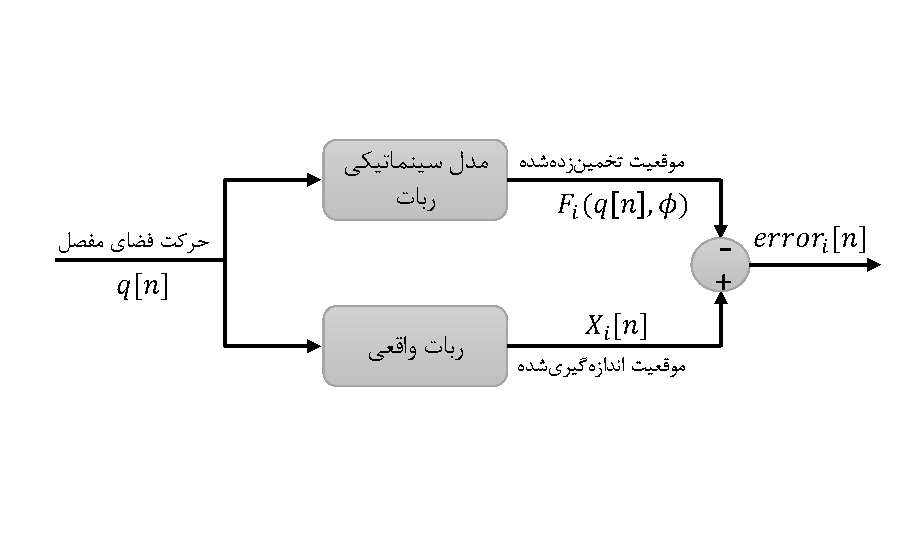
\includegraphics[width=0.8\linewidth, trim={0cm 2.2cm 0cm 2.2cm}, clip]{img/kinematic_model_error}
	\caption{}
	\label{fig:kinematicmodelerror}
\end{figure}


با نگاهی به آخرین تحقیقات بر روی مسئله کالیبراسیون ربات ها، ایجاد یک مسئله بهینه سازی غیرخطی و حل آن برای یافتن مقادیر دقیق این پارامتر های سینماتیکی و دینامیکی ربات مرسوم می باشد
\cite{elatta2004overview,ida2019automatic,ida2022identification,ida2021dynamics}.
مطابق این رویکرد های مروسم، برای ایجاد فرمول بندی مناسب مسئله مطرح شده در شکل \ref{fig:kinematicmodelerror} خواهیم داشت:

\begin{equation}\label{eq:optimization_equation_conventional}
	\tilde{\boldsymbol{\phi}} =  \arg\min_{\boldsymbol{\phi}} \sum_{n = 1 }^{N} \text{error}_i[n] = \arg\min_{\boldsymbol{\phi}} \sum_{n = 1}^{N} ||F_i(\boldsymbol{q}[n], \boldsymbol{\phi}) - X_i[n]||^2_{\Sigma}
\end{equation}

در این معادله، $\boldsymbol{\phi}$ بردار پارامتر های سینماتیکی و $\tilde{\boldsymbol{\phi}}$ تخمین آن است. علاوه بر این، $X_i[n]$، 
$iامین$
مقدار اندازه گیری شده توسط حسگر فضای کار ربات، و $\boldsymbol{q}[.]$ مقادیر اندازه گیری های متقابل حسگری در مفاصل می باشد. تابع مدل ربات $F[.]$ بیانگر مدل سینماتیک مستقیم ربات می باشد. تابع هزینه هدف، بر روی مجموعی از $N$ نمونه داده جمع آوری شده در فرآیند کالیبراسیون می باشد. افزون بر این، $\Sigma$ نیز بیانگر ماتریس کوواریانس اندازه گیری می باشد که به عنوان عامل نرمال سازی برای محاسبه هزینه عمل می کند. هر چه مقدار کوواریانس بیشتر باشد، میزان تاثیر گذاری خطای متقابل آن بر روی تابع هزینه کمتر خواهد بود. همچنین برای محاسبه نرم روش های زیادی ارائه شده است که آنچه بیشتر مورد استفاده قرار می گیرد نرم های هابر 
\footnote{\lr{Huber norms}}
می باشد
\cite{chang2015huber}.
معادله بهینه سازی غیر خطی بیان شده در 
\ref{eq:optimization_equation_conventional}
می تواند با روش های بازگشتی الگوریتم های غیر خطی حداقل مربعات
\footnote{\lr{Least-Square}}
همچون  لونبرگ-مارکوارت
\footnote{\lr{Levenberg Marquardt (LM)}}
و یا روش های گاوس-نیوتون
\footnote{\lr{Gauss-Newton(GN)}}
می باشد
\cite{dellart_robot_perception}.

با نگاهی دیگر به دیاگرام مطرح شده در 
\ref{fig:kinematicmodelerror}
و همچنین معادله 
\ref{eq:optimization_equation_conventional}،
مشاهده می‌شود که افزایش دقت اندازه‌گیری و همچنین برآورده کردن تمامی قیود مدل می‌تواند منجر به بهبود نتیجه کالیبراسیون شود. به منظور دستیابی به این هدف، رویکردهایی همچون ترکیب چندین حسگر و یا افزودن قیود جدید که از ساختار هندسی ربات استخراج می‌شود، معرفی می‌شوند. ترکیب این حسگرها باید به گونه‌ای باشد که علاوه بر کاهش خطای نهایی کالیبراسیون، خروج هر کدام از حسگرها منجر به توقف فرآیند کالیبراسیون نشود. همچنین واضح است که افزودن این قیود می‌تواند منجر به حل پیچیده‌تری از مسئله شود. در ادامه، نگاهی به فرمول‌بندی مسئله کالیبراسیون با در نظر گرفتن این ترکیب‌ها خواهیم داشت.

\subsubsection{ترکیب حسگر ها}
در معادله 
\ref{eq:optimization_equation_conventional}،
زیرنویس 
$i$
بیانگر وجود یک حسگر و خطایی که از مقادیر اندازه گیری حسگر در هر نمونه بوده می باشد. فرمول بندی ساختاری که به صورت همزمان از چندین حسگر در راستای ایجاد تابع هزینه استفاده نماید می تواند به صورت زیر تعریف شود:
\begin{equation}\label{eq:optimization_equation_conventional_multi_sensor}
	\tilde{\boldsymbol{\phi}} =  \arg\min_{\boldsymbol{\phi}} \sum_{n = 1 }^{N} \sum_{n = 1 }^{M} W_i~\text{error}_i[n] 
\end{equation}
در این معادله 
$W_i$
ها یک پارامتر وزن برای ترکیب چندین منبع اطلاعاتی با توجه به میزان کیفیت و اهمیت آنها می باشد.


\subsubsection{ترکیب شبه اندازه گیری ها}
اندازه گیری های حسگری تنها منبع اطلاعات برای حل مسئله نیستند. ساختار ربات و توحه به هندسه آن برای حل مسئله تعریف شده می تواند مفید واقع شود. برای مثال فاصله های بین برخی از نقاط می تواند با توجه به ساختار ربات می توانند ویژگی هایی نسبی و یا مطلق داشته باشند. این اطلاعات با عنوان داده های شبه اندازه گیری شناخته می شوند. این دسته از اطلاعات که از قبل مشخص هستند، می توانند به صورت قیود به مسئله اضافه شوند. بنابراین مسئله کلی بهینه سازی کالیبراسیون
\ref{eq:optimization_equation_conventional_multi_sensor}
در حضور این قیود به صورت زیر باز نویسی می شود. 
\begin{equation}
	\begin{aligned} \label{eq:optimization_equation_conventional_multi_sensor_measurement}
		&\tilde{\boldsymbol{\phi}} =  \arg\min_{\boldsymbol{\phi}} \sum_{n = 1 }^{N} \sum_{n = 1 }^{M} W_i~\text{error}_i[n] \\
		\quad &g_j(\boldsymbol{\phi}) = 0 \quad where \quad j = 1, \ldots, K
	\end{aligned}
\end{equation}
که در اینجا
$g_j(\boldsymbol{\phi}) = 0$ 
قیود هندسی معلوم بر روی پارامترهای سینماتیکی ربات می باشند.

\subsection{روش های مرسوم مسئله موقعیت یابی}
موقعیت یابی
\footnote{Localization}
 ربات فرآیند تعیین مکان ربات نسبت به محیط اطراف آن می باشد. دانستن موقعیت دقیق ربات در محیط، پیش‌نیازی اساسی برای اتخاذ تصمیمات صحیح و حرکت های بعدی مؤثر است. بدون اطلاعات موقعیتی دقیق، ربات نمی‌تواند مسیریابی
\footnote{motion planing}
  و یا ردیابی
\footnote{trakcing}
مناسبی را داشته باشد و ممکن است با موانع برخورد کند یا مسیر بهینه‌ای را طی نکند
\cite{ahmad2013cooperative}.
 علاوه بر این، سیستم‌های کنترلی ربات‌ها نیازمند اطلاعات دقیق و لحظه‌ای از موقعیت و جهت‌گیری ربات هستند تا بتوانند فرمان‌های مناسب را صادر کنند. بدون داده‌های دقیق موقعیتی، کنترلرها نمی‌توانند حرکات دقیقی را تولید کنند که منجر به عملکرد نامناسب و ناپایداری ربات می‌شود
\cite{guibas1997robot}.
فرآیند کالیبراسیون ربات که در بخش 
\ref{seq:conventional_calibration}
مورد بررسی قرار گرفت نیز یازمند داشتن اطلاعات دقیق از موقعیت ربات است. با داشتن داده‌های موقعیتی دقیق، می‌توان خطاهای سیستماتیک را شناسایی و تصحیح کرد و به این ترتیب دقت و کارایی ربات را بهبود بخشید. این امر به ویژه در ربات‌هایی که نیاز به انجام وظایف حساس و دقیق دارند، حیاتی است. 

موقعیت‌یابی دقیق ربات باعث کاهش عدم قطعیت در تصمیم‌گیری‌ها و عملیات ربات می‌شود. این امر نه تنها به افزایش اعتمادپذیری ربات در انجام وظایف محوله منجر می‌شود، بلکه احتمال بروز خطاها و حوادث ناشی از اشتباهات موقعیتی را نیز کاهش می‌دهد. همچنین در سیستم‌هایی که شامل چندین ربات هستند، اطلاعات دقیق موقعیتی هر ربات برای هماهنگی و همکاری بین ربات‌ها ضروری است. این اطلاعات به ربات‌ها کمک می‌کند تا از موقعیت یکدیگر آگاه باشند و بتوانند به صورت هماهنگ وظایف مشترک را انجام دهند. در این راستا توسعه و بهبود تکنیک‌های موقعیت‌یابی به منظور افزایش دقت و کارایی ربات‌ها، از اهمیت ویژه‌ای برخوردار است
\cite{aragues2011multi}.


روش های ارائه شده برای موقعیت یابی ربات را می توان به سه دسته اصلی مسافت پیمایی
\footnote{odometry}،
موقعیت یابی جهانی
\footnote{global localization}
و مکان یابی و نقشه یابی به صورت همزمان
تقسیم کرد. این روش ها با توجه به نوع حسگرهای تعبیه شده بر روی ربات می تواند مورد استفاده قرار گیرد. ترکیب داده ها برای همانند آنچه در بخش
\ref{seq:conventional_calibration}
\footnote{SLAM}
مورد توجه قرار گرفت، در موقعیت یابی و تخمین حالت ربات نیز می تواند نقش موثری را ایفا کند. حسگر های استفاده شده از نظر جنس داده ها و فرکانس داده برداری نیز می تواند متفاوت باشد که در ترکیب داده ها خصوصا زمانی که اجرای الگوریتم به صورت زمان واقعی می باشد، چالش برانگیز خواهد بود. طیف وسیعی از روش های مرسوم ارائه شده برای ترکیب داده ها در راستای تخمین حالت، رویکرد های بر مبنای فیلتر هستند. این روش ها که به رویکرهای آماری 
\footnote{stochastic}
نیز شناخته می شوند، در دو دهه اخیر فعالیت های زیادی را به خود اختصاص داده اند. پایه این روش ها بر قانون بیز
\footnote{Bayes law}
بنا نهاده شده است. مقاله
\cite{panigrahi2022localization} 
دسته بندی جامعی از روش های فیلتر مبنا برای تخمین موقعیت ارائه کرده است. از میان روش های بیان شده، کالمن فیلتر و فیلترهای ذرات
\footnote{particle filters}
به عنوان فراگیرترین رویکرد مورد استفاده قرار گرفته شده است. این فیلترها با استفاده از فرض مارکووی برای حالت ها و به کار گیری اطلاعات پیشین، تخمینی از حالت جدید ارائه می کنند. 

\subsection{رویکرد گراف مبنا برای حل مسئله کالیبراسیون و موقعیت یابی به صورت همزمان}
روش‌های مرسوم کالیبراسیون و موقعیت‌یابی ربات‌ها که تا به اینجا معرفی شده‌اند، فرمول‌بندی‌های مشخصی برای حل این دو مسئله ارائه داده‌اند. سادگی و سرعت بالای این روش‌ها باعث پیاده‌سازی گسترده آن‌ها، همانطور که در فصل قبل بحث شد، گردیده است. با این حال، این روش‌ها دارای معایبی نیز هستند. 
اول اینکه برای هر مسئله کالیبراسیون و ربات، فرمول‌بندی مسئله باید از ابتدا توسعه داده شود. دوم اینکه  این روش‌ها از تنک بودن ذاتی مسئله‌ها برای سرعت بخشیدن به محاسبات استفاده نمی‌کنند.  بزرگ شدن و پیچیده شدن فرمول‌بندی این مسائل باعث می‌شود که از حل آن‌ها به صورت زمان واقعی فاصله گرفته شود.  همچنین، این روش‌ها برای حل مسائل غیرخطی نیاز به خطی‌سازی دارند که نه تنها به پیچیدگی‌های محاسباتی می‌افزاید، بلکه باعث کاهش دقت نیز می‌شود. 
سومین موضوع،  روش‌های مرسوم فیلتر مبنا از داده‌های جاری و لحظه‌ای استفاده می‌کنند که باعث می‌شود علاوه بر مشکلات در مدیریت داده‌هایی که با تأخیر به سیستم می‌رسند، نتوانند داده‌های تاریخی را به صورت کامل در یک مسئله بهینه‌سازی دسته‌ای وارد کنند. این مشکل در مسائل موقعیت‌یابی باعث ایجاد مشکلات جدی همچون لغزش
\footnote{drift}
و کاهش دقت تا حد قابل توجهی می‌شود. چهارمین عیب این روش‌ها، عدم انعطاف‌پذیری آن‌ها برای بسط دادن مسئله با افزودن قیود به سیستم یا داده‌های حسگری به آن است. با توجه به این معایب، روش‌های مرسوم ممکن است در برخی کاربردهای پیشرفته رباتیک کارایی لازم را نداشته باشند. 

در این فصل، رویکردی گراف مبنا برای حل مسئله کالیبراسیون و موقعیت‌یابی ربات بیان می‌گردد که با یک فرمول‌بندی، هر دو مسئله را به صورت همزمان در یک مسئله بهینه‌سازی حل می‌کند. ویژگی‌های ذاتی این رویکرد در حل این مسئله واحد به تمامی معایب مطرح شده در روش‌های مرسوم پاسخ می‌دهد و باعث ایجاد حلی کامل و قابل بسط می‌شود. این رویکرد گراف مبنا به دلیل استفاده از ساختارهای گرافی، قادر به مدیریت بهینه‌تر داده‌های مختلف است. با ادغام تمامی داده‌های تاریخی و جاری در یک مسئله بهینه‌سازی دسته‌ای، این روش از داده‌های ورودی به صورت کامل استفاده کرده و به مشکلات مدیریت داده‌های تأخیر دار و لحظه‌ای غلبه می‌کند. همچنین، به دلیل عدم نیاز به خطی‌سازی مکرر، دقت محاسبات افزایش یافته و پیچیدگی‌های محاسباتی کاهش می‌یابد. علاوه بر این، انعطاف‌پذیری بالای این رویکرد امکان افزودن قیود و داده‌های حسگری جدید را فراهم می‌کند، بدون آن که نیاز به بازتعریف کلی فرمول‌بندی باشد. این ویژگی‌ها، در کنار توانایی بهره‌گیری از تنک بودن ذاتی مسئله‌ها برای بهینه‌سازی محاسبات، این رویکرد گراف مبنا را به یک ابزار قدرتمند برای کالیبراسیون و موقعیت‌یابی ربات‌ها تبدیل می‌کند.

الگوریتم گراف مبنای استفاده شده برای این فرمول‌بندی در این پایان‌نامه، الگوریتم گراف عامل
\footnote{factor graph}
می‌باشد. در ادامه، ابتدا نگاهی بر ریاضیات مرتبط با الگوریتم گراف عامل خواهیم داشت و سپس گراف عامل یکپارچه‌ای را برای حل مسئله مطرح شده معرفی خواهیم کرد. گراف عاملی که در ادامه پیشنهاد خواهد شد، حلی سیستماتیک برای کنار هم قرار دادن بلوک‌های ساختاری (عامل‌ها) در راستای تعریف یک مسئله کالیبراسیون در کنار مسئله موقعیت‌یابی به صورت یکپارچه است، که قابلیت گسترش به حسگرهای بیشتر و قیود اضافی را نیز دارا می‌باشد. علاوه بر این، از آنجایی که پیاده‌سازی‌های منابع باز و بهینه‌سازی شده برای این روش وجود دارد، مسئله کالیبراسیون و موقعیت‌یابی همزمان مطرح شده می‌تواند بر روی سیستم‌های نهفته بر روی ربات نیز پیاده‌سازی گردد. در این پایان‌نامه برای پیاده‌سازی گراف عامل پیشنهاد داده شده، از کتابخانه GTSAM استفاده شده است. 

\subsubsection{بیان الگوریتم گراف عامل}
الگوریتم گراف عامل بر پایه نظریه گراف‌ها و بهینه‌سازی به روش‌های مبتنی بر گراف توسعه یافته است. این الگوریتم به طور خاص برای حل مسائل بهینه‌سازی که شامل متغیرهای مختلف و قیود پیچیده است، طراحی شده است. یکی از روش‌های بیان، استفاده از نمودارهای دو بخشی
$F = (\mathcal{U}, \mathcal{V}, \mathcal{E})$
که  عامل‌ها 
$(\mathcal{U})$
با استفاده از یال‌ها
$(\mathcal{E})$
روابط و قیودی را بین گره‌ها 
$(\mathcal{V})$
 ایجاد می‌کنند. بدین ترتیب بخش اول، یعنی گره‌ها، نمایانگر متغیرهای ناشناخته یا پارامترهای مدل هستند که آنها را با
$\boldsymbol{\phi_i}$
نشان می‌دهیم. به عنوان مثال، در مسئله کالیبراسیون و موقعیت‌یابی، گره‌ها می‌توانند نمایانگر موقعیت‌های مختلف ربات یا پارامترهای کالیبراسیون باشند. همچنین بخش دوم، یعنی عامل‌ها، نشان‌دهنده قیود یا روابط بین متغیرها می‌باشد که آنها را با
$\psi_i$
نشان می‌دهیم. این قیود می‌توانند شامل معادلات غیرخطی یا روابط پیچیده‌ای باشند که باید در فرآیند بهینه‌سازی در نظر گرفته شوند. بدین ترتیب یک گراف عامل 
$F$
بیان کننده نحوه ایجاد یک تابع انرژی کلی
$\boldsymbol{\psi}$
از تک تک اجزای سیستم می باشد:
\begin{equation} 
	\boldsymbol{\psi}(\boldsymbol{\phi}) = \prod_{i} \boldsymbol{\psi}_i(\boldsymbol{\phi}_i) 
\end{equation}


\subsubsection{گراف عامل پیشنهادی برای کالیبراسیون و موقعیت یابی به صورت همزمان}
  
حل مسئله موقعیت یابی در انواع ربات ها به خوبی مورد بررسی قرار گرفته است. گراف عامل ایجاد شده 





\subsection{انتخاب ربات مناسب جهت توسعه  الگوریتم}
ربات نمونه انتخاب شده برای ارائه این فرمول بندی، یک ربات چهار کابلی فروتحریک آسان نصب می باشد. در این فصل حل کامل مسئله موقیت یابی و کالیبراسیون به صورت هزمان برای یک ربات کابلی فروتحریک با در نظر گرفتن فرض اساسی صلب بودن کابل ها مورد بررسی قرار می گیرد. علت انتخاب این نوع ربات آسان نصب به عنوان موضوع مورد بررسی، قابلیت استفاده زیاد آنها در کارکردهای متنوع رباتیکی می باشد به شرطی که هر بار پس از نصب در هر محیط دلخواه فرآیند کالیبراسیون بدون زمان بری و با کمترین زحمت انجام شود. فرمول بندی انجام شده برای این ربات به نحوی است که منجر به یک کالیبراسیون خودکار در کنار موقعیت یابی تنها با همان سنسور هایی که ربات برای موقعیت یابی تعبیه شده است بدون زحمت اضافی برای کاربر انجام می شود. نتیجه این رویکرد علاوه بر افزایش دقت نهایی این فرآیندها، مفهومی حقیقی تر به آسان نصب بودن به این دسته از ربات های کابلی می بخشد. 

صلب بودن کابل ها در حل این مسئله منجر می شود استفاده از این الگوریتم برای ربات هایی امکان پذیر باشد که نسبت جرم پنجه ربات به جرم کابل ها زیاد باشد به عبارتی دیگر میزان شکم دهی کابل ها قابل صرف نظر باشد. بزرگ شدن فضای کاری این ربات برای محیط هایی همچون یک استودیو فوتبال باعث ایجاد شکم دهی غیر قابل چشم پوشی می شود. بنابراین نیاز است فرمول بندی جدیدی ارائه شود که این شکم دهی را به خوبی مدلسازی کند. تا کنون تحقیقات زیادی برای توسعه این مدل انجام شده است و نتایج خوبی را برای این مدل سازی ارائه کرده اند. فرمول بندی های ارائه شده برای مدل بر مبنای توزیع نیرو در کابل ها می باشد که دارای پیچیدگی زیادی می باشند. به عبارتی افزودن این ویژگی کابل برای کالیبراسیون و موقعیت یابی یک ربات کابلی ضروری می باشد در حالی که میزان پیچیدگی حل مسئله به اندازه ای زیاد می شود که تا کنون برای محیط های بزرگ و کابل های شکم دار این موضوع مورد بررسی قرار نگرفته است. 

در ادامه این فصل، ابتدا فرمول بندی این مسئله برای یک ربات کابلی که کابل های آن صلب فرض می شود و حل می شود. در فصل آینده سپس با بزرگ کردن ابعاد ربات مسئله پیچیده ای را تعریف و فرمول بندی خواهیم کرد و سپس با گسترش دادن این رویکرد، مسئله جدید ایجاد شده که حل آن در روش های مرسوم کاری بسیار دشوار خواهد بود را حل خواهیم کرد. 
 

\subsection{توسعه گراف عامل برای یک ربات چهار کابلی فروتحریک با فرض کابل صلب}
 
 
 
 
 
 
 
 
 
 
 
 
 